\documentclass[tikz, dvipsnames]{report}
\usepackage{tikz, pgfplots}
    \pgfplotsset{compat=1.15}
\usetikzlibrary{intersections, math, decorations.markings, patterns}
\usepackage{circuitikz}
\usepackage{caption}
\usepackage{subcaption}
\usepackage{amsmath, bm}
\usepackage{tkz-tab}
\usepackage{graphicx}
\graphicspath{{figures/}}
\usepackage[showframe]{geometry}

\begin{document}

%%% excitation map
\begin{figure}[h]
    \tikzmath{\yone=1.3; \ytwo=2.5; \ythree=5;} 
    \centering
    \begin{subfigure}[b]{0.49\textwidth}
	\centering
	\begin{tikzpicture}
	    \centering
	    \begin{axis}[axis lines=middle,
		xmin=-1.4, xmax=2.75,
		ymin=0, ymax=7,
		xlabel={\large $k$},
		ylabel={\large$E$},
		xlabel style={below},
		xtick=\empty,
		ytick=\empty,
		x axis line style={draw=none},
		% clip=false,
		]
		\addplot[Violet, line width=3pt, samples=100, domain=-0.7:0.7, name path=A] {-2*x^2 + \yone};
		\addplot[OliveGreen, line width=3pt, samples=100, domain=-0.7:0.7, name path=B] {-2*x^2 + \ytwo};
		\addplot[OliveGreen, line width=3pt, samples=100, domain=-0.7:0.7, name path=B] {-1.2*x^2 + \ytwo};
		\addplot[Blue, line width=3pt, samples=100, domain=-0.7:0.7, name path=B] {2*x^2 + \ythree};
		\draw [/pgfplots/every inner x axis line, draw=black] (0,0) -- (\pgfkeysvalueof{/pgfplots/xmax}, 0); 
		\draw [dashed, draw=black] (0,\yone) -- (\pgfkeysvalueof{/pgfplots/xmax}, \yone);
		\draw [dashed, draw=black] (0,\ytwo) -- (\pgfkeysvalueof{/pgfplots/xmax}, \ytwo);
		\draw [dashed, draw=black] (0,\ythree) -- (\pgfkeysvalueof{/pgfplots/xmax}, \ythree);
		\draw [stealth-stealth, thick] (0.8, \yone) -- (0.8, \ytwo) node [midway, right] {\bm{$\Delta = 0.34\ eV$}};
		\draw [stealth-stealth, thick] (0.8, \ytwo) -- (0.8, \ythree) node [midway, right] {\bm{$E_{gap} = 1.42\ eV$}};
		\node [Violet, below] at (-1, \yone) {\large\bm{$P_{1/2}$}};
		\node [OliveGreen, below] at (-1, \ytwo) {\large\bm{$P_{3/2}$}};
		\node [Blue, above] at (-1, \ythree) {\large\bm{$S_{1/2}$}};
		\node [left, above] at (-0.2, \ytwo) {\large\bm{$E_F$}};
	    \end{axis}
	    \label{fg:excitation-a}
	\end{tikzpicture}
    \end{subfigure}
    \hfill
    \begin{subfigure}[b]{0.49\textwidth}
	\centering
	\begin{tikzpicture}
	    \begin{axis}[axis lines=middle,
		xmin=0, xmax=8,
		ymin=0, ymax=7,
		xlabel={\large $m_j$},
		ylabel={\large$E$},
		xlabel style={below},
		xtick=\empty,
		ytick=\empty,
		]
		\draw [/pgfplots/every inner y axis line, draw=black] (6.5,0) -- (6.5, \pgfkeysvalueof{/pgfplots/ymax}) node [below right] {\large J}; 
		\draw [draw=Violet, line width=2pt] (1.25,\yone) -- (2.25, \yone) node [midway, below, Violet] {\textbf{-1/2}};
		\draw [draw=Violet, line width=2pt] (4.25,\yone) -- (5.25, \yone) node [midway, below, Violet] {\textbf{+1/2}};
		\draw [draw=OliveGreen, line width=2pt] (0.5,\ytwo) -- (1.5, \ytwo) node [midway, below, OliveGreen] {\textbf{-3/2}};
		\draw [draw=OliveGreen, line width=2pt] (2,\ytwo) -- (3, \ytwo) node [midway, below, OliveGreen] {\textbf{-1/2}};
		\draw [draw=OliveGreen, line width=2pt] (3.5,\ytwo) -- (4.5, \ytwo) node [midway, below, OliveGreen] {\textbf{+1/2}};
		\draw [draw=OliveGreen, line width=2pt] (5,\ytwo) -- (6, \ytwo) node [midway, below, OliveGreen] {\textbf{+3/2}};
		\draw [draw=Blue, line width=2pt] (2,\ythree) -- (3, \ythree) node [midway, above, Blue] {\textbf{-1/2}};
		\draw [draw=Blue, line width=2pt] (3.5,\ythree) -- (4.5, \ythree) node [midway, above, Blue] {\textbf{+1/2}};
		\node [Violet, right] at (6.7, \yone-0.1) {\large\bm{$P_{1/2}$}};
		\node [OliveGreen, right] at (6.7, \ytwo-0.1) {\large\bm{$P_{3/2}$}};
		\node [Blue, right] at (6.7, \ythree-0.1) {\large\bm{$S_{1/2}$}};

		\draw [-stealth, Red, line width=2pt] (1, \ytwo) -- (2.5, \ythree) node [midway, circle, fill=CornflowerBlue, text=Black] {\textbf{3}};
		\draw [-stealth, Red, line width=2pt] (2.5, \ytwo) -- (4, \ythree);
		\node [above, Red] at (1, \ytwo+0.5) {\bm{$\sigma^+$}};
		\draw [-stealth, YellowOrange, line width=2pt] (4, \ytwo) -- (2.5, \ythree) node [midway, circle, fill=CornflowerBlue, text=Black] {\textbf{1}};
		\draw [-stealth, YellowOrange, line width=2pt] (5.5, \ytwo) -- (4, \ythree) node [midway, circle, fill=CornflowerBlue, text=Black] {\textbf{3}};
		\node [above, YellowOrange] at (5.5, \ytwo+0.5) {\bm{$\sigma^-$}};
	    \end{axis}
	\end{tikzpicture}
	\label{fg:excitation-b}
    \end{subfigure}
    \caption{Excitation of polarized electrons}
\end{figure}

%%% GaAs energy band diagram
\begin{figure}
    \centering
    \begin{subfigure}[b]{0.49\textwidth}
	\tikzmath{\yone=2.5; \ytwo=6; \ythree=9.5;} 
	\centering
	\begin{tikzpicture}
	    \centering
	    \begin{axis}[axis lines=middle,
		xmin=-3, xmax=1,
		ymin=0, ymax=10,
		hide axis,
		]
		\draw [dashed] (-1, \yone) -- (0, \yone);
		\draw [dashed] (-1, \ytwo) -- (0, \ytwo);
		\draw [dashed] (\pgfkeysvalueof{/pgfplots/xmin}, \ythree) -- (\pgfkeysvalueof{/pgfplots/xmax}, \ythree);
		\draw [Violet, line width=2pt] (0, 0) -- (0, \ythree) -- (\pgfkeysvalueof{/pgfplots/xmax}, \ythree);
		\draw [Violet, line width=2pt] (\pgfkeysvalueof{/pgfplots/xmin}, \yone)  -- (-0.5, \yone) arc (90:0:0.5);
		\draw [Violet, line width=2pt] (\pgfkeysvalueof{/pgfplots/xmin}, \ytwo)  -- (-0.5, \ytwo) arc (90:0:0.5);
		\draw [stealth-stealth, thick] (\pgfkeysvalueof{/pgfplots/xmin} + 1, \yone) -- (\pgfkeysvalueof{/pgfplots/xmin} + 1, \ytwo) node [midway, left] {\bm{$E_{gap}$}};
		\draw [stealth-stealth, thick, Red] (-0.5, \ytwo) -- (-0.5, \ythree) node [midway, left] {\textbf{PEA = 4.07 eV}};
		\node [Red, above left] at (0, 0) {\textbf{GaAs}};
		\node [Red, above right] at (0, 0) {\textbf{Vaccum}};
		\node [below left, text width=2cm] at (-0.3, \yone) {\textbf{Valance Band}};
		\node [below left, text width=2cm] at (-0.3, \ytwo) {\textbf{Conduction Band}};
	    \end{axis}
	\end{tikzpicture}
	\label{fg:PEA}
    \end{subfigure}
    \hfill
    \begin{subfigure}[b]{0.49\textwidth}
	\tikzmath{\yone=2.5; \ytwo=6; \ythree=5;} 
	\centering
	\begin{tikzpicture}
	    \centering
	    \begin{axis}[axis lines=middle,
		xmin=-2, xmax=4.5,
		ymin=0, ymax=10,
		hide axis,
		]
		\draw [dashed] (\pgfkeysvalueof{/pgfplots/xmin}, \yone) -- (\pgfkeysvalueof{/pgfplots/xmax}, \yone);
		\draw [dashed] (\pgfkeysvalueof{/pgfplots/xmin}, \ytwo) -- (\pgfkeysvalueof{/pgfplots/xmax}, \ytwo);
		\draw [dashed] (\pgfkeysvalueof{/pgfplots/xmin}, \ythree) -- (\pgfkeysvalueof{/pgfplots/xmax}, \ythree);
		\draw [Violet, line width=2pt] (0, 0) -- (0, 9.5) -- (0.3, \ythree-0.5) arc (180:90:0.5) -- (\pgfkeysvalueof{/pgfplots/xmax}, \ythree);
		\draw [Violet, line width=2pt] (\pgfkeysvalueof{/pgfplots/xmin}+0.5, \yone)  -- (-0.5, \yone) arc (90:0:0.5);
		\draw [Violet, line width=2pt] (\pgfkeysvalueof{/pgfplots/xmin}+0.5, \ytwo)  -- (-0.5, \ytwo) arc (90:0:0.5);
		\draw [stealth-stealth, thick, Red] (\pgfkeysvalueof{/pgfplots/xmax}/3, \ytwo) -- (\pgfkeysvalueof{/pgfplots/xmax}/3, \ythree) node [midway, right] {\textbf{NEA = 0.2 eV}};
		\node [Red, above left] at (0, 0) {\textbf{GaAs}};
		\node [Red, above right] at (0, 0) {\textbf{Vaccum}};
		\node (e1) at (\pgfkeysvalueof{/pgfplots/xmin}/2, \yone)[circle, fill=CornflowerBlue, text=Black] {\textbf{e}};
		\node (e2) at (\pgfkeysvalueof{/pgfplots/xmin}/2, \ytwo)[circle, fill=CornflowerBlue, text=Black] {\textbf{e}};
		\node (e3) at (\pgfkeysvalueof{/pgfplots/xmax}/4, \ythree)[circle, fill=CornflowerBlue, text=Black] {\textbf{e}};
		\draw [-stealth, thick, CornflowerBlue] (e1) -- (e2);
		\draw [-stealth, thick, CornflowerBlue] (e2) -- (e3);
		\node (light) at (\pgfkeysvalueof{/pgfplots/xmax}/4*3, \yone+0.5) {};
		\draw [-stealth, thick, YellowOrange] (light) node [above, sloped, YellowOrange] {\textbf{Light}} -- (e1) ;
	    \end{axis}
	\end{tikzpicture}
	\label{fg:NEA}
    \end{subfigure}
    \caption{Left: energy band diagram of bare GaAs, the large positive 
    electron affinity (PEA) prevent electrons from escaping the surface; Right: 
    energy band diagram of GaAs with Oxided Cs, the electron vaccum energy is
    lowered so that the electron affinity is negative now.}
\end{figure}

%%% a more complete plot
\begin{figure}
    \centering
    \begin{subfigure}[b]{0.32\textwidth}
	\tikzmath{\yone=2.5; \ytwo=5; \ythree=9.5;} 
	\centering
	\resizebox{\textwidth}{0.33\textheight}{
	\begin{tikzpicture}
	    \centering
	    \begin{axis}[
		axis lines=middle,
		xmin=-3, xmax=1,
		ymin=0, ymax=10,
		hide axis,
		]
		\draw [dashed] (\pgfkeysvalueof{/pgfplots/xmin}, \yone) -- (0, \yone) node [right] {\bm{$E_F$}};
		\draw [dashed] (\pgfkeysvalueof{/pgfplots/xmin}, \ytwo) -- (0, \ytwo);
		\draw [dashed] (\pgfkeysvalueof{/pgfplots/xmin}, \ythree) -- (0, \ythree);
		\draw [Violet, line width=2pt] (0, 0) -- (0, \ythree) -- (\pgfkeysvalueof{/pgfplots/xmax}/4, \ythree) node [right, Black] {\bm{$E_\infty$}};
		\fill [pattern=north east lines] (\pgfkeysvalueof{/pgfplots/xmin}, \yone)  -- (-1, \yone) arc (90:0:1) -- (0, 0) -- (\pgfkeysvalueof{/pgfplots/xmin}, 0) -- (\pgfkeysvalueof{/pgfplots/xmin}, \yone);
		\draw [Violet, line width=2pt] (\pgfkeysvalueof{/pgfplots/xmin}, \yone)  -- (-1, \yone) arc (90:0:1);
		\draw [Violet, line width=2pt] (\pgfkeysvalueof{/pgfplots/xmin}, \ytwo)  -- (-1, \ytwo) arc (90:0:1);
		\draw [stealth-stealth, thick] (\pgfkeysvalueof{/pgfplots/xmin} + 0.8, \yone) -- (\pgfkeysvalueof{/pgfplots/xmin} + 0.8, \ytwo) node [midway, left] {\bm{$E_{gap}$}};
		\draw [stealth-stealth, thick, Red] (-0.5, \ytwo) -- (-0.5, \ythree) node [midway, left] {\textbf{PEA = 4.07 eV}};
		\node [Red, above] at (\pgfkeysvalueof{/pgfplots/xmin}/2, 0) {\textbf{GaAs}};
		\node [Red, above right] at (0, 0) {\textbf{Vac}};
		\node [below left, text width=2cm] at (-0.5, \yone) {\textbf{Valance Band}};
		\node [below left, text width=2cm] at (-0.5, \ytwo) {\textbf{Conduction Band}};
	    \end{axis}
	\end{tikzpicture}
	}
    \end{subfigure}
    \hfill
    \begin{subfigure}[b]{0.32\textwidth}
	\tikzmath{\yone=2.5; \ytwo=5; \ythree=9.5;} 
	\centering
	\resizebox{\textwidth}{0.33\textheight}{
	\begin{tikzpicture}
	    \centering
	    \begin{axis}[
		axis lines=middle,
		xmin=-3, xmax=1,
		ymin=0, ymax=10,
		hide axis,
		]
		\draw [dashed] (\pgfkeysvalueof{/pgfplots/xmin}, \yone) -- (0, \yone) node [right] {\bm{$E_F$}};
		\draw [dashed] (\pgfkeysvalueof{/pgfplots/xmin}, \ytwo) -- (0, \ytwo);
		\node at (0, \pgfkeysvalueof{/pgfplots/ymax}) {};
		\draw [OliveGreen, line width=5pt] (-0.07, 0) -- (-0.07, \ytwo);
		\draw [Violet, line width=2pt] (0, 0) -- (0, \ytwo) -- (\pgfkeysvalueof{/pgfplots/xmax}/4, \ytwo) node [right, Black] {\bm{$E_\infty$}};
		\fill [pattern=north east lines] (\pgfkeysvalueof{/pgfplots/xmin}, \yone)  -- (-1, \yone) arc (90:0:1) -- (0, 0) -- (\pgfkeysvalueof{/pgfplots/xmin}, 0) -- (\pgfkeysvalueof{/pgfplots/xmin}, \yone);
		\draw [Violet, line width=2pt] (\pgfkeysvalueof{/pgfplots/xmin}, \yone)  -- (-1, \yone) arc (90:0:1);
		\draw [Violet, line width=2pt] (\pgfkeysvalueof{/pgfplots/xmin}, \ytwo)  -- (-1, \ytwo) arc (90:0:1);
		\node [Red, above] at (\pgfkeysvalueof{/pgfplots/xmin}/2, 0) {\textbf{GaAs}};
		\node [Red, above] at (-0.03, 0) {\textbf{Cs}};
		\node [Red, above right] at (0.1, 0) {\textbf{Vac}};
	    \end{axis}
	\end{tikzpicture}
	}
    \end{subfigure}
    \hfill
    \begin{subfigure}[b]{0.32\textwidth}
	\tikzmath{\yone=2.5; \ytwo=5; \ythree=4; \surface=0.8;} 
	\centering
	\resizebox{\textwidth}{0.33\textheight}{
	\begin{tikzpicture}
	    \centering
	    \begin{axis}[
		axis lines=middle,
		xmin=-3, xmax=1,
		ymin=0, ymax=10,
		hide axis,
		]
		\draw [dashed] (\pgfkeysvalueof{/pgfplots/xmin}, \yone) -- (0, \yone) node [right] {\bm{$E_F$}};
		\draw [dashed] (\pgfkeysvalueof{/pgfplots/xmin}, \ytwo) -- (0, \ytwo);
		\draw [dashed] (\pgfkeysvalueof{/pgfplots/xmin}, \ythree) -- (0, \ythree);
		\node at (0, \pgfkeysvalueof{/pgfplots/ymax}) {};
		\draw [Violet, line width=2pt] (0, 0) -- (0, \ythree) -- (\pgfkeysvalueof{/pgfplots/xmax}/4, \ythree) node [right, Black] {\bm{$E_\infty$}};
		\fill [pattern=north east lines] (\pgfkeysvalueof{/pgfplots/xmin}, \yone)  -- (-1-\surface, \yone) arc (90:0:1) -- (-\surface, 1.4) arc (180:270:\surface) --  (0, 0) -- (\pgfkeysvalueof{/pgfplots/xmin}, 0) -- (\pgfkeysvalueof{/pgfplots/xmin}, \yone);
		\draw [Violet, line width=2pt] (-\surface, 0) -- (-\surface, \ytwo/2 + \ythree/2) arc (180:270:\surface);
		\draw [Violet, line width=2pt] (-\surface, 1.4) arc (180:270:\surface);
		\draw [Violet, line width=2pt] (\pgfkeysvalueof{/pgfplots/xmin}, \yone)  -- (-1-\surface, \yone) arc (90:0:1);
		\draw [Violet, line width=2pt] (\pgfkeysvalueof{/pgfplots/xmin}, \ytwo)  -- (-1-\surface, \ytwo) arc (90:0:1);
		\node [Red, above] at (\pgfkeysvalueof{/pgfplots/xmin}/2, 0) {\textbf{GaAs}};
		\node [Red, above] at (-0.4, 0) {\bm{$Cs_2O$}};
		\node [Red, above right] at (0.1, 0) {\textbf{Vac}};

		\node (e1) at (\pgfkeysvalueof{/pgfplots/xmin}/5*3, \yone)[circle, fill=CornflowerBlue, text=Black] {\textbf{e}};
		\node (e2) at (\pgfkeysvalueof{/pgfplots/xmin}/5*3, \ytwo)[circle, fill=CornflowerBlue, text=Black] {\textbf{e}};
		\node (e3) at (0.2, \ythree*1.1)[circle, fill=CornflowerBlue, text=Black] {\textbf{e}};
		\draw [-stealth, thick, CornflowerBlue] (e1) -- (e2);
		\draw [-stealth, thick, CornflowerBlue] (e2) -- (e3);
		\draw [stealth-stealth, thick, Red] (-2.2, \ytwo) -- (-2.2, \ythree) node [midway, left] {\textbf{NEA}};
	    \end{axis}
	\end{tikzpicture}
	}
    \end{subfigure}
\end{figure}
    
\begin{figure}[h]
    \begin{tikzpicture}
	\begin{scope}
	    \node[anchor=south west, inner sep=0] (image) at (0, 0)
	    {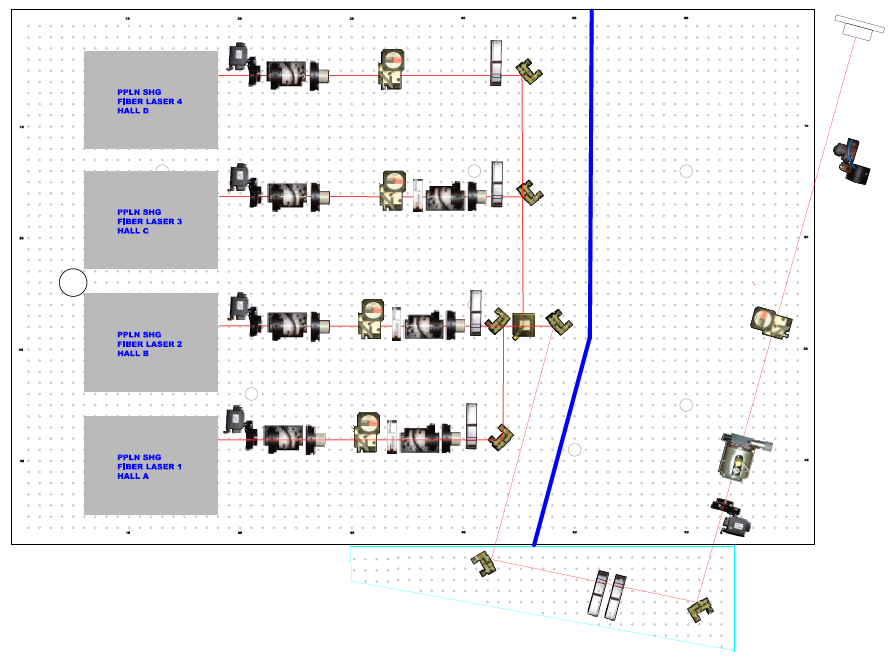
\includegraphics[width=\linewidth]{laser_table};
	    \begin{scope}[x={(image.south east)},y={(image.north west)}]
		\draw[red,ultra thick] (0.435,0.435) circle (0.17 cm);
		\draw [-latex, thick, red] (0.46, 0.1) node {\scriptsize{Pinch Point}} -- (0.44,0.39);
		\node[green] (coll) at (0.7, 0.2) {\scriptsize{Collimator}};
		\draw [-latex, thick, green] (coll.north) -- (0.67,0.51);
	    \end{scope}
	\end{scope}
    \end{tikzpicture}
\end{figure}

%%% laser table
\begin{figure}[h]
    \begin{tikzpicture}
	\tikzstyle{explain} = [align=center] 
	\begin{scope}
	    \node[anchor=south west, inner sep=0] (image) at (0, 0)
	    {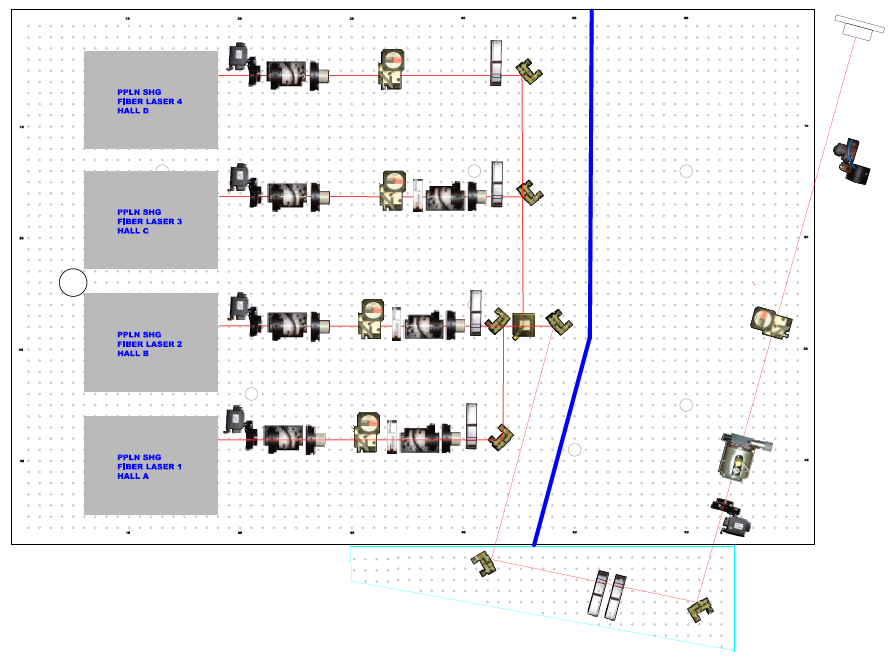
\includegraphics[width=\linewidth]{laser_table}};
	    \begin{scope}[x={(image.south east)},y={(image.north west)}]
		\node [blue,ultra thick] at (0.06,0.3) {\textbf{A}};
		\node [blue,ultra thick] at (0.06,0.49) {\textbf{B}};
		\node [blue,ultra thick] at (0.06,0.67) {\textbf{C}};
		\node [blue,ultra thick] at (0.06,0.85) {\textbf{D}};

		\node [blue,ultra thick] at (0.47,0.39) {\textbf{IA}};
		\node [blue,ultra thick] at (0.47,0.56) {\textbf{IA}};
		\node [blue,ultra thick] at (0.5,0.75) {\textbf{IA}};

		\node [red] at (0.75,0.23) {\textbf{IHWP}};
		\node [explain,red] at (0.76,0.33) {\textbf{Pockels } \\ \textbf{Cell}};
		\node [red] at (0.8,0.53) {\textbf{RHWP}};
		\node [explain,red] at (0.88, 0.96) {\textbf{Beamline} \\ \textbf{vaccum} \\ \textbf{window}};
	    \end{scope}
	\end{scope}
    \end{tikzpicture}
\end{figure}
\end{document}
